
%(BEGIN_QUESTION)
% Copyright 2015, Tony R. Kuphaldt, released under the Creative Commons Attribution License (v 1.0)
% This means you may do almost anything with this work of mine, so long as you give me proper credit

Suppose a pair of current transformers with 600:5 ratios are parallel-connected to feed their output signals to a protective relay as shown in this schematic diagram:

$$\includegraphics[width=15.5cm]{i02872x01.eps}$$

\begin{itemize}
\item{} $R_{CT}$ = 0.5 $\Omega$ (this is the internal resistance of each CT's secondary winding)
\item{} $R_{relay}$ = 1.8 $\Omega$
\end{itemize}

\vskip 10pt

Calculate the following voltage drops in this current transformer circuit, from the given information:

\begin{itemize}
\item{} $V_{relay}$ = \underbar{\hskip 50pt} volts
\vskip 5pt
\item{} Voltage output at each CT's terminals = \underbar{\hskip 50pt} volts 
\vskip 5pt
\item{} Voltage generated by each CT's secondary winding (before any $R_{CT}$ losses) = \underbar{\hskip 50pt} volts 
\end{itemize}

\vskip 20pt \vbox{\hrule \hbox{\strut \vrule{} {\bf Suggestions for Socratic discussion} \vrule} \hrule}

\begin{itemize}
\item{} Sketch current arrows showing the direction of each CT's secondary current relative to the direction shown for the 137 amp primary current.
\item{} Explain why the two CT secondary windings must be paralleled as shown, and not parallel-connected with one of the CT's polarity reversed.
\end{itemize}

\underbar{file i02872}
%(END_QUESTION)





%(BEGIN_ANSWER)

 
%(END_ANSWER)





%(BEGIN_NOTES)

First, we must know how much current is being output by each CT.  With a primary current of 137 amps and a ratio of 600:5, each CT will output:

$$I_{CT} = \left({137 \hbox{ A} \over 1} \right) \left({5 \over 600} \right) = 1.1417 \hbox{ A}$$

Note how both CTs are paralleled such that their currents sum together to power the protective relay.  This means the protective relay sees an input current of 2.2833 amps ($I_{relay} = I_{CT} + I_{CT}$).

Now that we know the value for $I_{relay}$, calculating voltage drop is a simple matter of applying Ohm's Law ($V = IR$):

$$V_{relay} = I_{relay} R_{relay} = (2.2833 \hbox{ A})(1.8 \> \Omega) = 4.110 \hbox{ V}$$

Voltage at each CT's terminals is identical to voltage dropped across the protective relay terminals, since both CTs are parallel to the relay with negligible wire resistance in between.  Therefore, $V_{CT-terminals}$ = 4.110 volts.

\vskip 10pt

The amount of voltage produced internally by each CT winding is simply the terminal voltage (4.110 volts) plus whatever is dropped by the internal winding resistance.  This internal winding drop may be found via Ohm's Law, given the current output by each CT and its wire resistance:

$$V_{R_{CT}} = I_{CT} R_{CT} = (1.1417 \hbox{ A})(0.5 \> \Omega) = 0.5708 \hbox{ V}$$

Internal CT winding voltage is therefore equal to:

$$V_{CT-winding} = V_{CT-terminals} + I_{CT} R_{CT} = 4.110 \hbox{ V} + 0.5708 \hbox{ V} = 4.6808 \hbox{ V}$$


%INDEX% Electronics review: current transformer (CT)
%INDEX% Protective relay: CT circuit wire resistance

%(END_NOTES)


